\documentclass[journal,12pt,twocolumn]{IEEEtran}

\usepackage{setspace}
\usepackage{gensymb}
\singlespacing
\usepackage[cmex10]{amsmath}

\usepackage{amsthm}

\usepackage{mathrsfs}
\usepackage{txfonts}
\usepackage{stfloats}
\usepackage{bm}
\usepackage{cite}
\usepackage{cases}
\usepackage{subfig}

\usepackage{longtable}
\usepackage{multirow}

\usepackage{enumitem}
\usepackage{mathtools}
\usepackage{steinmetz}
\usepackage{tikz}
\usepackage{circuitikz}
\usepackage{verbatim}
\usepackage{tfrupee}
\usepackage[breaklinks=true]{hyperref}
\usepackage{graphicx}
\usepackage{tkz-euclide}

\usetikzlibrary{calc,math}
\usepackage{listings}
    \usepackage{color}                                            %%
    \usepackage{array}                                            %%
    \usepackage{longtable}                                        %%
    \usepackage{calc}                                             %%
    \usepackage{multirow}                                         %%
    \usepackage{hhline}                                           %%
    \usepackage{ifthen}                                           %%
    \usepackage{lscape}     
\usepackage{multicol}
\usepackage{chngcntr}

\DeclareMathOperator*{\Res}{Res}

\renewcommand\thesection{\arabic{section}}
\renewcommand\thesubsection{\thesection.\arabic{subsection}}
\renewcommand\thesubsubsection{\thesubsection.\arabic{subsubsection}}

\renewcommand\thesectiondis{\arabic{section}}
\renewcommand\thesubsectiondis{\thesectiondis.\arabic{subsection}}
\renewcommand\thesubsubsectiondis{\thesubsectiondis.\arabic{subsubsection}}


\hyphenation{op-tical net-works semi-conduc-tor}
\def\inputGnumericTable{}                                 %%

\lstset{
%language=C,
frame=single, 
breaklines=true,
columns=fullflexible
}
\begin{document}


\newtheorem{theorem}{Theorem}[section]
\newtheorem{problem}{Problem}
\newtheorem{proposition}{Proposition}[section]
\newtheorem{lemma}{Lemma}[section]
\newtheorem{corollary}[theorem]{Corollary}
\newtheorem{example}{Example}[section]
\newtheorem{definition}[problem]{Definition}

\newcommand{\BEQA}{\begin{eqnarray}}
        \newcommand{\EEQA}{\end{eqnarray}}
\newcommand{\define}{\stackrel{\triangle}{=}}
\bibliographystyle{IEEEtran}
\raggedbottom
\setlength{\parindent}{0pt}
\providecommand{\mbf}{\mathbf}
\providecommand{\pr}[1]{\ensuremath{\Pr\left(#1\right)}}
\providecommand{\qfunc}[1]{\ensuremath{Q\left(#1\right)}}
\providecommand{\sbrak}[1]{\ensuremath{{}\left[#1\right]}}
\providecommand{\lsbrak}[1]{\ensuremath{{}\left[#1\right.}}
\providecommand{\rsbrak}[1]{\ensuremath{{}\left.#1\right]}}
\providecommand{\brak}[1]{\ensuremath{\left(#1\right)}}
\providecommand{\lbrak}[1]{\ensuremath{\left(#1\right.}}
\providecommand{\rbrak}[1]{\ensuremath{\left.#1\right)}}
\providecommand{\cbrak}[1]{\ensuremath{\left\{#1\right\}}}
\providecommand{\lcbrak}[1]{\ensuremath{\left\{#1\right.}}
\providecommand{\rcbrak}[1]{\ensuremath{\left.#1\right\}}}
\theoremstyle{remark}
\newtheorem{rem}{Remark}
\newcommand{\sgn}{\mathop{\mathrm{sgn}}}
\providecommand{\abs}[1]{\left\vert#1\right\vert}
\providecommand{\res}[1]{\Res\displaylimits_{#1}}
\providecommand{\norm}[1]{\left\lVert#1\right\rVert}
%\providecommand{\norm}[1]{\lVert#1\rVert}
\providecommand{\mtx}[1]{\mathbf{#1}}
\providecommand{\mean}[1]{E\left[ #1 \right]}
\providecommand{\fourier}{\overset{\mathcal{F}}{ \rightleftharpoons}}
%\providecommand{\hilbert}{\overset{\mathcal{H}}{ \rightleftharpoons}}
\providecommand{\system}{\overset{\mathcal{H}}{ \longleftrightarrow}}
%\newcommand{\solution}[2]{\textbf{Solution:}{#1}}
\newcommand{\solution}{\noindent \textbf{Solution: }}
\newcommand{\cosec}{\,\text{cosec}\,}
\providecommand{\dec}[2]{\ensuremath{\overset{#1}{\underset{#2}{\gtrless}}}}
\newcommand{\myvec}[1]{\ensuremath{\begin{pmatrix}#1\end{pmatrix}}}
\newcommand{\mydet}[1]{\ensuremath{\begin{vmatrix}#1\end{vmatrix}}}
\numberwithin{equation}{subsection}

\makeatletter
\@addtoreset{figure}{problem}
\makeatother
\let\StandardTheFigure\thefigure
\let\vec\mathbf

\renewcommand{\thefigure}{\theproblem}

\def\putbox#1#2#3{\makebox[0in][l]{\makebox[#1][l]{}\raisebox{\baselineskip}[0in][0in]{\raisebox{#2}[0in][0in]{#3}}}}
\def\rightbox#1{\makebox[0in][r]{#1}}
\def\centbox#1{\makebox[0in]{#1}}
\def\topbox#1{\raisebox{-\baselineskip}[0in][0in]{#1}}
\def\midbox#1{\raisebox{-0.5\baselineskip}[0in][0in]{#1}}
\vspace{3cm}
\title{Assignment 1}
\author{V. L. Narasimha Reddy - EE18BTECH11046}
\maketitle
\newpage
\bigskip
\renewcommand{\thefigure}{\theenumi}
\renewcommand{\thetable}{\theenumi}
Download all python codes from
\begin{lstlisting}
https://github.com/narasimha-123/EE4013/tree/main/Assignment-1/codes
\end{lstlisting}
%
and latex-tikz codes from
%
\begin{lstlisting}
https://github.com/narasimha-123/EE4013/tree/main/Assignment-1/figs
\end{lstlisting}
\section{Problem}
Consider the following C program
\begin{lstlisting}
#include <stdio.h>

struct OurNode
{
    char x, y, z;
};

int main()
{
    struct OurNode p = {'0', '1', 'a' + 2};
    struct OurNode *q = &p;
    printf("%c,%c \n", *((char *)q + 1), *((char *)q + 2));
}
\end{lstlisting}

The output of the following program is

\section{Solution}

The output of the given C program we get is
\begin{lstlisting}
    1,c
\end{lstlisting}

In the code, We are defining a new structure using struct.
\begin{lstlisting}
struct OurNode
{
    char x, y, z;
};
\end{lstlisting}

A struct is a composite data type (or record) declaration that defines a
physically grouped list of variables under one name in a block of memory,
allowing the different variables to be accessed via a single pointer or
by the struct declared name which returns the same address.

%The memory block created using the above struct will look like this:
\begin{figure}[!ht]
    \begin{center}
        \resizebox{\columnwidth}{!}{%\begin{figure}


% The block diagram code is probably more verbose than necessary
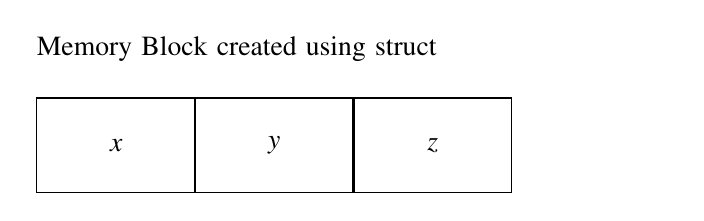
\begin{tikzpicture}[auto, node distance=3cm,>=latex']
    % Controller
    \node [draw,
        minimum width=2cm,
        minimum height=1.2cm
    ]  (Memory1) at (0,0) {$x$};
    \node [draw,
        minimum width=2cm,
        minimum height=1.2cm,
        right=0cm of Memory1
    ]  (Memory2) {$y$};
    \node [draw,
        minimum width=2cm,
        minimum height=1.2cm,
        right=0cm of Memory2
    ]  (Memory3) {$z$};
    \node[text width=8cm, anchor=north] at (3,1.5)
    {Memory Block created using struct};

\end{tikzpicture}
%\end{figure
}
    \end{center}
    \caption{Memory block created using Struct OurNode}
    \label{fig:ee18btech11046_memeory}
\end{figure}


As part of code the data types defined in the struct are same(char). So we can also assume this
as a char array of size 3 in a single continuous block of memory.

Initially we created a block of memory  using the struct and assigned
three chars $'0','1','a'+2$ as values in memory fields. Then a pointer $p$ is created to
store the address value of the first char element of the struct.
\begin{lstlisting}
    struct OurNode p = {'0', '1', 'a' + 2};
\end{lstlisting}

Since the field members of the struct are chars, $'a'+2$ is stored as char $'c'$.

The struct created along with pointer pointing to the first element ia as shown below:
\begin{figure}[!ht]
    \begin{center}
        \resizebox{\columnwidth}{!}{\input{./figs/ee18btech11046_2.tex}}
    \end{center}
    \caption{struct OurNode $p$}
    \label{fig:ee18btech11046_memeory2}
\end{figure}


Then we are creating a new pointer $q$ and assigning it the address of previously created struct $p$.
So new pointer $q$ stores the address of the first element in struct $p$.
\begin{lstlisting}
    struct OurNode *q = &p;
\end{lstlisting}
The new pointer $q$ points to the same memory address as that of pointer $p$
\begin{figure}[!ht]
    \begin{center}
        \resizebox{\columnwidth}{!}{%\begin{figure}


% The block diagram code is probably more verbose than necessary
\begin{tikzpicture}[auto, node distance=3cm,>=latex']
    % Controller
    \node [draw,
        minimum width=2cm,
        minimum height=1.2cm
    ]  (Memory1) at (0,0) {$0$};
    \node [draw,
        minimum width=2cm,
        minimum height=1.2cm,
        right=0cm of Memory1
    ]  (Memory2) {$1$};
    \node [draw,
        minimum width=2cm,
        minimum height=1.2cm,
        right=0cm of Memory2
    ]  (Memory3) {$c$};
    \node [draw,
        minimum width=1cm,
        minimum height=1cm,
        below left= 2cm and 0.5cm of Memory1
    ] (Pointer1) {$p$};
    \node [draw,
        minimum width=1cm,
        minimum height=1cm,
        below left= 2cm and -1.5cm of Memory1
    ] (Pointer2) {$q$};
    % Arrows with text label
    \draw[-stealth] (Pointer1.north) -- (Memory1.south west)
    node[midway,above]{};
    \draw[-stealth] (Pointer2.north) -- (Memory1.south)
    node[midway,above]{};

\end{tikzpicture}
%\end{figure
}
    \end{center}
    \caption{OurNode $p$ with pointer $q$}
    \label{fig:ee18btech11046_memeory3}
\end{figure}

Now $q+1$ points to the address of the next element from the pointer $q$ and similarlly
$q+2$ points to the next address from the pointer $q+1$.
\begin{figure}[!ht]
    \begin{center}
        \resizebox{\columnwidth}{!}{%\begin{figure}


% The block diagram code is probably more verbose than necessary
\begin{tikzpicture}[auto, node distance=3cm,>=latex']
    % Controller
    \node [draw,
        minimum width=2cm,
        minimum height=1.2cm
    ]  (Memory1) at (0,0) {$0$};
    \node [draw,
        minimum width=2cm,
        minimum height=1.2cm,
        right=0cm of Memory1
    ]  (Memory2) {$1$};
    \node [draw,
        minimum width=2cm,
        minimum height=1.2cm,
        right=0cm of Memory2
    ]  (Memory3) {$c$};
    % \node [draw,
    %     minimum width=1cm,
    %     minimum height=1cm,
    %     below left= 2cm and -0.25cm of Memory1
    % ] (Pointer1) {$p$};
    \node [draw,
        minimum width=1cm,
        minimum height=1cm,
        below left= 2cm and -0.7cm of Memory2
    ] (Pointer2) {$q+1$};
    \node [draw,
        minimum width=1cm,
        minimum height=1cm,
        below left= 2cm and -0.7cm of Memory3
    ] (Pointer3) {$q+2$};
    % Arrows with text label
    % \draw[-stealth] (Pointer1.north) -- (Memory1.south)
    % node[midway,above]{};
    \draw[-stealth] (Pointer2.north) -- (Memory2.south)
    node[midway,above]{};
    \draw[-stealth] (Pointer3.north) -- (Memory3.south)
    node[midway,above]{};

\end{tikzpicture}
%\end{figure
}
    \end{center}
    \caption{pointers $q+1$ and $q+2$}
    \label{fig:ee18btech11046_memeory4}
\end{figure}

\begin{lstlisting}{language=C}
    printf("%c,%c \n", *((char *)q + 1), *((char *)q + 2))
    \end{lstlisting}

So, now the above printf line prints the element stored at the address $q+1$ and $q+2$ points
in the terminal i.e., \textbf{1}, \textbf{c}.



\end{document}